\documentclass[11pt,a4paper]{article}
\usepackage[T1]{fontenc}
\usepackage{lmodern}
\usepackage[margin=24mm,headheight=15pt]{geometry}
\usepackage{amsmath,amssymb,mathtools,bm}
\allowdisplaybreaks[2]
\usepackage{booktabs,tabularx,longtable,array,graphicx}
\usepackage[dvipsnames]{xcolor}
\usepackage{tikz}
\usetikzlibrary{arrows.meta,positioning,fit,calc}
\usepackage[most]{tcolorbox}
\usepackage{enumitem,fancyhdr,titlesec,microtype}
\usepackage[hyphens]{url}
\usepackage[colorlinks=true,linkcolor=RoyalBlue,citecolor=RoyalBlue,urlcolor=RoyalBlue,
 pdftitle={World Models, Contact Geometry, and Useful Policy Gradients},
 pdfauthor={IsaacLab research literature review},bookmarksnumbered=true]{hyperref}
\definecolor{ink}{HTML}{14263D}
\definecolor{blue}{HTML}{2563EB}
\definecolor{green}{HTML}{0F766E}
\definecolor{orange}{HTML}{B45309}
\setlength{\parindent}{0pt}
\setlength{\parskip}{0.5em}
\setlength{\emergencystretch}{3em}
\renewcommand{\arraystretch}{1.15}
\renewcommand{\tabularxcolumn}[1]{>{\raggedright\arraybackslash}p{#1}}
\newcolumntype{L}[1]{>{\raggedright\arraybackslash}p{#1}}
\setlist{leftmargin=*,itemsep=0.25em,topsep=0.3em}
\titleformat{\section}{\Large\bfseries\color{ink}}{\thesection}{0.7em}{}
\titleformat{\subsection}{\large\bfseries\color{ink}}{\thesubsection}{0.7em}{}
\pagestyle{fancy}\fancyhf{}
\fancyhead[L]{\small World models, contact geometry, and useful policy gradients}
\fancyfoot[L]{\small\color{gray}Focused literature review / November 9, 2026}
\fancyfoot[R]{\thepage}
\newtcolorbox{keyidea}[1]{colback=blue!4,colframe=blue!60,title={#1},
 fonttitle=\bfseries,boxrule=0.5pt,arc=2pt,breakable}
\newtcolorbox{interpretation}[1]{colback=green!4,colframe=green!65,title={#1},
 fonttitle=\bfseries,boxrule=0.5pt,arc=2pt,breakable}
\newtcolorbox{limitation}[1]{colback=orange!4,colframe=orange!65,title={#1},
 fonttitle=\bfseries,boxrule=0.5pt,arc=2pt,breakable}
\newcommand{\R}{\mathbb R}
\newcommand{\E}{\mathbb E}
\newcommand{\sg}{\operatorname{sg}}
\newcommand{\KL}{D_{\mathrm{KL}}}
\newcommand{\TV}{D_{\mathrm{TV}}}
\newcommand{\norm}[1]{\left\lVert#1\right\rVert}
\newcommand{\code}[1]{\texttt{\small\detokenize{#1}}}
\newcommand{\loc}[1]{\par{\footnotesize\color{gray}\raggedright Source locator: #1.\par}}
\newcommand{\Fsim}{F_{\mathrm{sim}}}
\newcommand{\Fhat}{\widehat F_\phi}
\newcommand{\Hhist}{\mathcal H}
\newcommand{\Gtask}{\mathcal G}
\newcommand{\policy}{\pi_\theta}
\tikzset{box/.style={draw=blue!55,fill=blue!4,rounded corners=2pt,align=center,
 minimum height=10mm,font=\small,inner sep=4pt},
 arr/.style={-{Latex[length=2mm]},thick,draw=ink},
 grad/.style={-{Latex[length=2mm]},thick,dashed,draw=orange}}
\begin{document}
\hypersetup{pageanchor=false}
\begin{titlepage}
\vspace*{12mm}
{\color{blue}\large A FOCUSED MATHEMATICAL LITERATURE REVIEW}\par
\vspace{8mm}
{\Huge\bfseries\color{ink}World Models,\\Contact Geometry,\\and Useful Policy Gradients}\par
\vspace{8mm}
{\Large From learned motion dynamics to adaptation under new contacts}\par
\vspace{10mm}
\begin{keyidea}{The research question}
How much additional interaction is needed to adapt a motion-pretrained world
model to new contact geometry, and what model structure makes its gradients
useful for control?
\end{keyidea}
\vspace{5mm}
This review develops one notation, examines eleven selected papers, and separates
three questions: predicting physical outcomes, obtaining useful optimization
directions, and transferring knowledge to a new environment.
\par
\vspace{6mm}
\begin{tabularx}{\linewidth}{@{}lX@{}}
Coverage & Foundational work from 2018--2022 and directly relevant work from 2025--2026\\
Recent anchors & PWM, DMO, RWM-U, SuperMimic, $\nabla$Mimic, and WM-LOCO\\
Foundations & PETS, MBPO, Dreamer, ContactNets, and SHAC\\
Scope & Robot dynamics, contact structure, policy learning, terrain information,
and measurable adaptation cost\\
Prepared & November 9, 2026\\
\end{tabularx}
\vfill
{\small Primary papers are cited with version and section/equation locators.
Mathematics is restated in a common notation rather than copied verbatim.
Critical interpretations, illustrative derivations, and proposed experiments
are explicitly distinguished from published findings. No new training result
or claim of novelty is asserted by this review.}
\end{titlepage}
\hypersetup{pageanchor=true}
\tableofcontents
\clearpage
\section{Scope, evidence, and how to read the review}
The central object is a model that predicts how a controlled robot evolves. The
proposed transfer problem changes the contact geometry after pretraining that
model on a motion library. A successful research result would explain both the
additional data needed and the reliability of the policy updates obtained from
the adapted model.

The eleven papers were selected because each isolates a necessary part of that
question. PETS concerns uncertainty and planning; MBPO concerns how much model
rollout to trust; Dreamer concerns learned latent dynamics and imagination;
ContactNets concerns contact structure; SHAC concerns short simulator-gradient
windows. PWM, DMO, RWM-U, SuperMimic, $\nabla$Mimic, and WM-LOCO make the more direct
connections to learned gradients, humanoid motion, and terrain-aware control.

This is a question-driven selection, not an exhaustive survey. General video
generation, language-conditioned robot foundation models, and broad motion
retargeting surveys are outside its scope. A model that predicts photorealistic
video is not automatically a model with adequate action sensitivity for motor control.

Each paper is treated using the same sequence: its role, a concise account of
the reported method, a normalized mathematical skeleton, an analysis of what
that skeleton means, and a test or limitation relevant to contact transfer.
The analysis is original to this review; it should not be mistaken for an
experiment performed by the cited authors.

\begin{limitation}{Evidence discipline}
No reviewed result establishes the number of interactions required for our exact
flat-motion-to-new-stair-geometry experiment. That quantity depends on the
source data, target distribution, observations, controller, model class, and
success criterion. A reported wall-clock speedup on motion tracking cannot
substitute for this missing measurement.
\end{limitation}

Read Sections~\ref{sec:notation}--\ref{sec:contactproblem} first. For the most
direct path, continue with PWM, DMO, SuperMimic, $\nabla$Mimic, and WM-LOCO.
The earlier papers explain the model-usage and representation choices behind
them. Sections~\ref{sec:comparison}--\ref{sec:experiments} turn the review into
an experimental question.

\section{One notation for all methods}\label{sec:notation}
\subsection{Physical state, environment, task, and observations}
Let $x_t$ be the physical state of the robot and any moving objects included in
the system. Static environmental geometry is $E$; material, calibration, and
other physical parameters are $\xi$. The transition is
\begin{equation}\label{eq:true}
x_{t+1}\sim P_{E,\xi}(\cdot\mid x_t,a_t),\qquad
x_{t+1}=\Fsim(x_t,a_t;E,\xi)\quad\text{when deterministic}.
\end{equation}
Here $a_t$ is the action actually executed, after any exploration noise and
clipping. An explicit actuation map $u_t=\mathcal U(a_t)$ converts it to a physical
setpoint or torque when needed. Numerical comparisons must specify whether
action coordinates are normalized values, radians, or torques.
If an implementation predicts an offset relative to a reference, we include
the reference addition inside the policy and call its resulting executed command
$a_t$. The model must receive the command that actually determines actuation;
an offset alone is insufficient when its reference-dependent baseline is unknown.
$\mathcal U$ is an actuator map, while $M(q)$ below always denotes a mass matrix.

Write $\Gtask_t$ for the complete task/reference specification, including its
phase where relevant. The supplied policy-goal vector is
$g_t=G(x_t,\Gtask_t)$. This distinction matters: a compact actor goal can omit
reference quantities still used by the training reward. We associate reward
$r_t$ with the transition $t\rightarrow t+1$:
\begin{equation}
r_t=R(x_t,a_t,x_{t+1};\Gtask_t,E),\qquad
o_t\sim O(\cdot\mid x_t,E,\xi).
\end{equation}
Papers that call this reward $r_{t+1}$ have simply shifted the label in this review.
The observation/action history is $\Hhist_t$. A geometry query or perceptual
encoder supplies local environment information $e_t$:
\begin{equation}
e_t=\mathcal Q(E,x_t)\ \text{with known geometry},\qquad
e_t=\mathcal E_\phi(\Hhist_t)\ \text{when inferred}.
\end{equation}
The same terrain map must be queried at the predicted pose during imagination.
Using future simulator observations inside a learned rollout would change the
information available to the algorithm.

\subsection{Network roles and probability conventions}
\begin{longtable}{@{}L{0.22\linewidth}L{0.73\linewidth}@{}}
\toprule Symbol & Meaning throughout this review\\\midrule\endhead
$\theta$ & Policy parameters, including task encoders/projections assigned to the policy.\\
$\phi$ & Learned dynamics, observation encoders, and predictive heads.\\
$\psi$ & Value-function parameters; $\bar\psi$ denotes a target copy.\\
$\policy$ & Policy, deterministic or reparameterized stochastic as specified.\\
$\Fhat$ & Learned physical-state transition or transition mean.\\
$\widehat P_\phi$ & Learned transition distribution.\\
$z_t=(m_t,\ell_t)$ & Learned latent state: deterministic memory and stochastic component when present.\\
$\mathsf q_\phi$ & Observation-conditioned posterior over a latent state.\\
$\mathsf p_\phi$ & Latent transition prior, propagated without the next observation.\\
$\widehat R_\phi$ & Learned reward predictor, when the algorithm uses one.\\
$\zeta_t$ & Learned motion-goal embedding, distinct from actuator command $u_t$.\\
$V_\psi,Q_\psi$ & State-value and action-value functions.\\
$\gamma,\lambda$ & Discount and lambda-return mixing coefficient.\\
$c_t,C_t$ & One-step continuation and cumulative continuation, $C_t=\prod_{i<t}c_i$.\\
$\sg(\cdot)$ & Stop-gradient: preserve a value but suppress that derivative path.\\
$H,K$ & Policy-optimization horizon and model-fitting horizon, respectively.\\
$N_{\rm pre},N_{\rm new}$ & Pretraining and additional target-environment transitions.\\
\bottomrule
\end{longtable}
Parameter labels denote roles, not a requirement that implementations have
three disjoint optimizers. An actor and critic may share a trunk. The policy's
input may be $x_t$, a history, or $z_t$; using the same $\theta$ does not erase
those architectural differences.

We always call an observation-conditioned latent distribution a posterior
$\mathsf q_\phi$ and a prediction-only distribution a prior $\mathsf p_\phi$.
This reverses the letters used by the original Dreamer paper, intentionally;
the distinction is stated again in its method section. Contact impulses are
$j$, not $\lambda$, so they cannot be confused with the return coefficient.

\subsection{State models versus latent models}
A physical-state model uses
\begin{equation}
\hat x_{t+1}=\Fhat(\hat x_t,a_t,e_t,\xi).
\end{equation}
A latent model instead infers a posterior from observations and rolls a prior:
\begin{align}
z_t&\sim\mathsf q_\phi(z_t\mid z_{t-1},a_{t-1},o_t),\\
\hat z_{t+1}&\sim\mathsf p_\phi(z_{t+1}\mid\hat z_t,a_t).
\end{align}
Some inputs are absent in a particular paper. We never infer that a method uses
terrain conditioning merely because $e_t$ appears in this general template.
A task embedding, an environment encoding, and a belief over unobserved
physical parameters are three different kinds of conditioning.

\section{A common mathematical lens for learning and control}\label{sec:common}
\subsection{Fitting dynamics}
A physical model can be trained by negative log likelihood,
\begin{equation}\label{eq:nll}
L_{\rm dyn}(\phi)=-\E_{\mathcal D}\log\widehat P_\phi(x_{t+1}\mid x_t,a_t,e_t,\xi),
\end{equation}
or a multistep residual loss. With $\hat x_0=x_0$ and logged actions,
\begin{equation}\label{eq:multistep}
L_{\rm dyn}^{(K)}=\E_{\mathcal D}\sum_{k=0}^{K-1}w_k
\norm{\Delta(x_{k+1},\hat x_{k+1})}_{W}^{2},\quad
\hat x_{k+1}=\Fhat(\hat x_k,a_k,e_k,\xi).
\end{equation}
$\Delta$ must respect the state representation: quaternion coordinates should
not be treated as unconstrained Euclidean angles. A latent model may instead
learn observation/reward likelihoods and a prior--posterior consistency term.

These objectives measure predictions on a data distribution. They do not
directly certify errors at policy-chosen states outside that distribution or
derivatives of those predictions.

\subsection{Short-horizon actor--critic as the common backbone}
Let $y_t$ temporarily mean the optimization state: $x_t$ for a physical-state
model and $z_t$ for a latent model. This is a placeholder, not an extra latent.
Many methods use a variant of
\begin{equation}\label{eq:shortobjective}
J_H=\E\left[\sum_{t=0}^{H-1}\gamma^t C_t\widetilde r_t
+\gamma^H C_HV_\psi(y_H,g_H)\right],
\end{equation}
where $\widetilde r_t$ can be an analytic reward or a learned prediction.
Continuation can be hard termination or a soft surrogate. Reference-end masks
are an additional implementation detail, not implied by this notation.

One useful normalized value target is
\begin{align}\label{eq:lambda}
Y_H&=V_\psi(y_H,g_H),\\
Y_t&=\widetilde r_t+\gamma c_t\big[(1-\lambda)V_\psi(y_{t+1},g_{t+1})+\lambda Y_{t+1}\big],\\
L_V&=\E\big[V_\psi(y_t,g_t)-\sg(Y_t)\big]^2.
\end{align}
This template does not claim identical target networks, reward normalization,
discount indexing, or terminal handling in every method. Such differences are
identified in the paper analyses.

\subsection{Four different ways a model can enter control}
\begin{enumerate}
\item \textbf{Planning}: score candidate actions under model rollouts and select
one, without differentiating a neural policy through the model.
\item \textbf{Imagined policy optimization}: generate predicted trajectories and
differentiate their return with respect to policy parameters.
\item \textbf{Decoupled forward/backward}: use physical-simulator states in the
forward pass and learned local Jacobians in the backward pass.
\item \textbf{Predictive features}: feed a learned recurrent representation to
a policy trained by another estimator, such as PPO.
\end{enumerate}
These choices should be compared separately from the choice of state versus
latent representation. ``Uses a world model'' is not a complete algorithm description.

\begin{figure}[htbp]
\centering
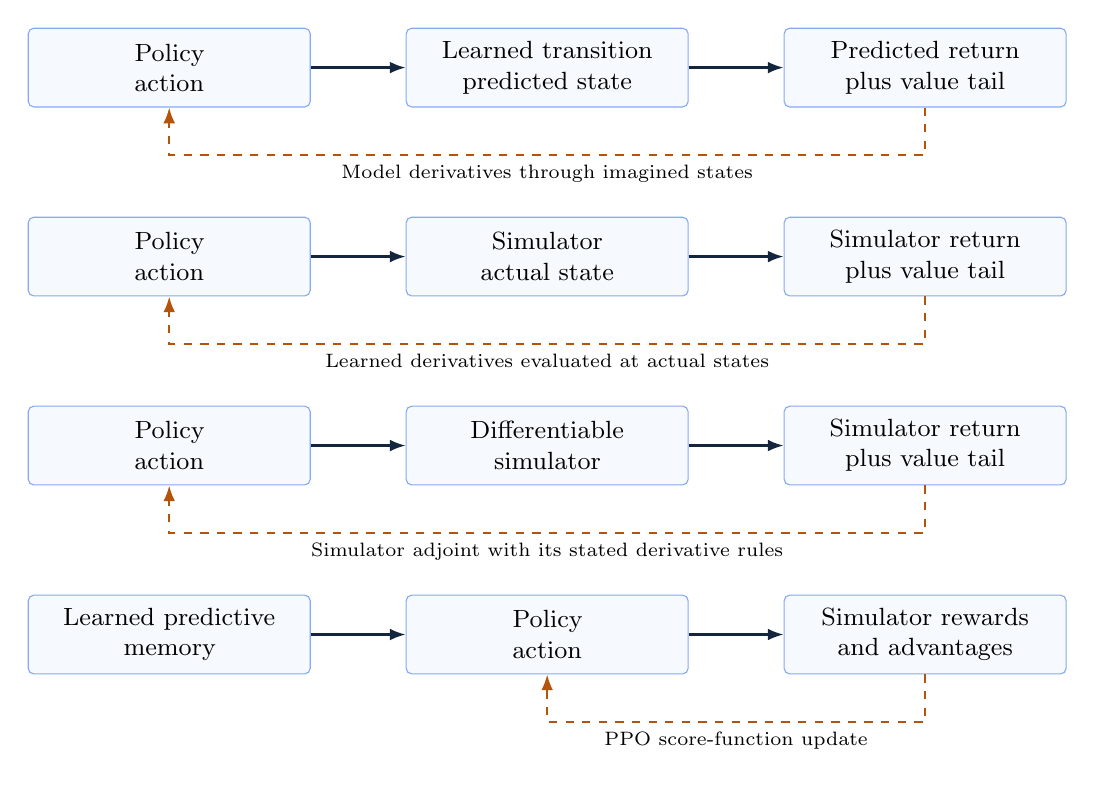
\begin{tikzpicture}
\node[box,text width=33mm] (a) at (0,0) {Policy\\action};
\node[box,text width=33mm] (b) at (4.8,0) {Learned transition\\predicted state};
\node[box,text width=33mm] (c) at (9.6,0) {Predicted return\\plus value tail};
\draw[arr](a)--(b);\draw[arr](b)--(c);
\draw[grad](c.south)--++(0,-0.6)-|node[pos=0.25,below,font=\scriptsize]{Model derivatives through imagined states}(a.south);
\node[box,text width=33mm] (d) at (0,-2.4) {Policy\\action};
\node[box,text width=33mm] (e) at (4.8,-2.4) {Simulator\\actual state};
\node[box,text width=33mm] (f) at (9.6,-2.4) {Simulator return\\plus value tail};
\draw[arr](d)--(e);\draw[arr](e)--(f);
\draw[grad](f.south)--++(0,-0.6)-|node[pos=0.25,below,font=\scriptsize]{Learned derivatives evaluated at actual states}(d.south);
\node[box,text width=33mm] (g) at (0,-4.8) {Policy\\action};
\node[box,text width=33mm] (h) at (4.8,-4.8) {Differentiable\\simulator};
\node[box,text width=33mm] (i) at (9.6,-4.8) {Simulator return\\plus value tail};
\draw[arr](g)--(h);\draw[arr](h)--(i);
\draw[grad](i.south)--++(0,-0.6)-|node[pos=0.25,below,font=\scriptsize]{Simulator adjoint with its stated derivative rules}(g.south);
\node[box,text width=33mm] (j) at (0,-7.2) {Learned predictive\\memory};
\node[box,text width=33mm] (k) at (4.8,-7.2) {Policy\\action};
\node[box,text width=33mm] (l) at (9.6,-7.2) {Simulator rewards\\and advantages};
\draw[arr](j)--(k);\draw[arr](k)--(l);
\draw[grad](l.south)--++(0,-0.6)-|node[pos=0.25,below,font=\scriptsize]{PPO score-function update}(k.south);
\end{tikzpicture}
\caption{Four policy-learning routes. Solid arrows show forward information;
dashed arrows label the update estimator. The final row uses advantages and
action log probabilities, not differentiation of simulator reward through the
dynamics. Inputs and repeated rollout steps are omitted for readability.}
\end{figure}

\subsection{A derivative is an additional modeling requirement}
For a deterministic policy at a fixed task schedule, suppress other inputs and
write $a_t=A_\theta(x_t)$. The pathwise sensitivity is
\begin{equation}\label{eq:sensitivity}
D_\theta x_{t+1}=(F_x+F_aA_x)D_\theta x_t+F_aA_\theta.
\end{equation}
The matrices $F_x,F_a$ come from a simulator or a learned function. History,
latent memory, and state-dependent goal construction can be included by
augmenting the optimization state. Freezing $\phi$ during the actor update
does not remove $\partial\Fhat/\partial a$ or $\partial\Fhat/\partial x$.
When $e=\mathcal Q(E,x)$, the total state derivative also includes the geometry
query path where that path is differentiable. A discrete query requires a
declared piecewise derivative or surrogate; silently dropping it changes the update.

This equation identifies two independent failure paths: the forward states can
be wrong, or the local sensitivities can be wrong even at good forward states.
Products of sensitivities can amplify errors as $H$ grows.

\begin{interpretation}{Original illustration: small prediction error, large derivative error}
Consider $F(a)=a$ and $\widehat F(a)=a+\epsilon\sin(\omega a)$. Prediction error
is at most $\epsilon$, yet derivative error can reach $\epsilon\omega$. Taking
$\epsilon=0.01$ and $\omega=200$ gives at most 0.01 state error and derivative
error as large as two. The predicted derivative can even point in the opposite
direction. This elementary construction is not an empirical result from a
reviewed paper; it explains why a trajectory-fit metric alone cannot certify
useful policy gradients.
\end{interpretation}
\begin{figure}[htbp]\centering
\includegraphics[width=\linewidth]{figures/prediction_and_gradient.pdf}
\caption{Synthetic review illustration of the distinction between prediction
and derivative errors. No paper measurements are plotted.}
\end{figure}

\section{What changes when the contact geometry changes?}\label{sec:contactproblem}
\subsection{The missing-input problem}
For two environments $E_1,E_2$, identical $(x,a)$ can yield
\begin{equation}
\Fsim(x,a;E_1,\xi)\ne\Fsim(x,a;E_2,\xi).
\end{equation}
A model with no environment information cannot distinguish those outcomes in
general. A larger network cannot recover information that its inputs omit.
With one fixed known map and suitable global coordinates, location can encode
geometry implicitly; that is not generalization to arbitrary unseen maps.

Flat-ground motion already involves impacts, support changes, slipping, and
body contacts. The proposed transfer changes \emph{which surfaces exist and
where they are}, potentially also which body parts touch them. Later tasks may
change friction, compliance, object motion, or contact laws as well. Those are
distinct axes and should not be changed simultaneously in the first experiment.

\subsection{An idealized contact template}
For configuration $q$ and generalized velocity $v$, a rigid-contact template is
\begin{align}\label{eq:mechanics}
M(q)(v_{t+1}-v_t)&=\Delta t\,f_{\rm free}(x_t,u_t)+J(q,E)^Tj_t,\\
q_{t+1}&\approx q_t+\Delta t\,\Gamma(q_t)v_{t+1},\\
d_i(q_{t+1},E)&\ge0,\quad j_i^n\ge0,\quad d_i(q_{t+1},E)j_i^n=0,\\
\norm{j_i^\tau}&\le\mu_i j_i^n.
\end{align}
$d_i$ is signed distance, $J$ maps generalized to contact-frame velocity, and
$j$ is impulse. $\Gamma$ handles configuration representations such as floating-base
quaternions. Complementarity says contact pushes only at an active surface.
This is an explanatory rigid-contact template, not a claim that every reviewed
simulator uses exactly this forward law; compliant contact models differ.

When contact identities or modes change, a derivative taken with the current
active set may not explain the effect of a finite action change that creates a
different contact. Simulator exactness, hardware fidelity, and usefulness for
optimization are consequently separate questions.

\subsection{What a terrain-aware imagined rollout must maintain}
If $e_t$ is an egocentric map, advancing $\hat x_t$ requires advancing the map
query or predicting the relevant latent scene. Holding an arbitrary local
encoding constant while the robot moves can give inconsistent predictions.
For moving objects, their states must be modeled too. For hidden materials or
occluded geometry, a history-dependent belief may be necessary.

The task must also remain coherent. Tracking a world-aligned flat-ground
reference while climbing may penalize the correct height increase. Terrain-aware
dynamics alone does not repair a mismatched goal, reward, critic input, or
termination rule. These distinctions guide the paper selection that follows.

\section{PETS: uncertainty-aware dynamics for planning}\label{sec:pets}
\textbf{Chua et al., 2018.} Deep Reinforcement Learning in a Handful of Trials
using Probabilistic Dynamics Models~\cite{pets}.
\loc{Sections 4--5; probabilistic ensembles, trajectory sampling, and MPC}

\subsection{Reported mechanism in common notation}
PETS fits bootstrapped probabilistic neural dynamics models and propagates
particles through them to evaluate candidate action sequences. Model differences
represent epistemic uncertainty; each model's predicted distribution represents
transition uncertainty. Control uses sampling-based model predictive control,
executing the first selected action and replanning. This is a model-based
planning method, not policy BPTT through a learned simulator.

For model index $b=1,\ldots,B$, the normalized predictive form is
\begin{align}
\widehat P_{\phi_b}(x'\mid x,a)&=\mathcal N\big(x+\mu_{\phi_b}(x,a),
\Sigma_{\phi_b}(x,a)\big),\\
L_b&=\E_{\mathcal D_b}\left[
(\Delta x-\mu_b)^T\Sigma_b^{-1}(\Delta x-\mu_b)+\log\det\Sigma_b\right].
\end{align}
Constants and a common factor of one half are omitted. $\mathcal D_b$ is a
bootstrap sample; the covariance is diagonal in the neural parameterization.
Particle propagation and the finite planning objective can be written
\begin{align}
\hat x_{k+1}^{(p)}&\sim\widehat P_{\phi_{b_{p,k}}}(\cdot\mid\hat x_k^{(p)},a_k),\\
a_{t:t+H-1}^{*}&\approx\arg\max_{a_{t:t+H-1}}
\frac1P\sum_p\sum_{k=0}^{H-1}\gamma^k r(\hat x_k^{(p)},a_k),\\
a_t^{\rm execute}&=a_t^*.
\end{align}
Resampling ensemble identity across steps and retaining it along a particle
are different trajectory-sampling choices. The latter preserves a coherent
model hypothesis through a rollout.

\subsection{What the formulation exposes}
For an equally weighted ensemble, the law of total variance gives
\begin{equation}\label{eq:ensemblevariance}
\operatorname{Var}(x')=\frac1B\sum_b\Sigma_b
+\frac1B\sum_b(\mu_b-\bar\mu)(\mu_b-\bar\mu)^T.
\end{equation}
The first term describes spread inside a model; the second describes disagreement
between models. A deterministic network with an uncertainty score bolted onto
its output is therefore not equivalent to this construction.

Equation~\eqref{eq:ensemblevariance} is a useful design lens, not a calibration
guarantee. If every model ignores a stair riser, all can agree on the same wrong
prediction. If geometry is missing from the input, variance can instead represent
different unobserved environments producing different outcomes. Measuring that
spread does not tell the controller where the obstacle actually is.

There is also a control distinction. Candidate-action search can evaluate
sequences across different predicted outcomes without using $\partial\Fhat/\partial a$.
A derivative-based policy can fail even when such a planner succeeds, or vice
versa. Comparing them distinguishes model quality from gradient usability.

\subsection{Relevance to adaptation and a discriminating experiment}
Use an ensemble as an uncertainty baseline for the new-geometry problem. On
held-out stair contacts, measure whether disagreement ranks actual prediction
errors and failed control updates. Report reliability curves by contact type,
not just a global correlation. In particular, test examples with unseen riser
height and examples with an unseen collision orientation separately.

An uncertainty-gated controller should be compared with an ungated controller
under the same interaction budget, including any extra samples the gate requests.
The research question is whether uncertainty identifies when additional contact
data is useful. Calling the ensemble ``uncertainty aware'' alone does not answer it.

\section{MBPO: controlling the amount of model-generated experience}\label{sec:mbpo}
\textbf{Janner et al., 2019.} When to Trust Your Model: Model-Based Policy
Optimization~\cite{mbpo}.
\loc{Sections 4--5; practical algorithm and branched-rollout analysis}

\subsection{Reported mechanism in common notation}
MBPO learns an ensemble transition/reward model from real experience, starts
short model rollouts from replay states, and trains a model-free policy using
the generated transitions. The practical implementation uses SAC. Its central
choice is the amount of model usage, rather than differentiating a policy through
many learned transition steps. Real collection and model learning continue online.

Let $\mathcal D_{\rm real}$ and $\mathcal D_{\rm model}$ denote replay sources:
\begin{align}
x_0&\sim\mathcal D_{\rm real},\quad a_k\sim\policy(\cdot\mid\hat x_k),\\
(\hat x_{k+1},\hat r_k)&\sim\widehat P_\phi^{x,r}(\cdot\mid\hat x_k,a_k),
\qquad 0\le k<h_{\rm roll},\\
\mathcal D_{\rm model}&\leftarrow\mathcal D_{\rm model}\cup
\{(\hat x_k,a_k,\hat r_k,\hat x_{k+1})\}.
\end{align}
The superscript $x,r$ explicitly denotes a joint state/reward predictor;
$\widehat P_\phi$ without it continues to mean the state-transition distribution.
A soft actor--critic update on the chosen replay mixture has the standard skeleton
\begin{align}
y_t&=r_t+\gamma c_t\E_{a'\sim\policy}
\left[\min_iQ_{\bar\psi_i}(x_{t+1},a')-\alpha\log\policy(a'\mid x_{t+1})\right],\\
L_Q&=\sum_i\E\big[Q_{\psi_i}(x_t,a_t)-\sg(y_t)\big]^2,\\
L_\pi&=\E_{x,a\sim\policy}\left[\alpha\log\policy(a\mid x)-\min_iQ_{\psi_i}(x,a)\right].
\end{align}
The actor differentiates through the critic's action input, not through a chain
of $\Fhat$ Jacobians. These equations express the estimator distinction; they
do not reproduce every replay or target-update hyperparameter.

\subsection{An original coupling argument for short rollouts}
The following is a review derivation, not MBPO's published policy-improvement
theorem. Fix a policy, environment, and initial-state distribution. For this argument only, use the same
bounded current-state reward $|r(x,a)|\le R_{\max}$ in both systems and assume a
uniform transition error $\TV(P,\widehat P)\le\varepsilon$ on every visited input.
Couple the two trajectories so each step remains matched with probability at
least $1-\varepsilon$. By a union bound,
\begin{equation}
\Pr[x_t\ne\hat x_t]\le\min(1,t\varepsilon).
\end{equation}
When the states disagree, their rewards differ by at most $2R_{\max}$, giving
\begin{equation}\label{eq:coupling}
|J_H-\widehat J_H|\le2R_{\max}\sum_{t=0}^{H-1}\gamma^t\min(1,t\varepsilon).
\end{equation}
If a learned reward also has uniformly bounded error $\varepsilon_r$, add
$\varepsilon_r\sum_t\gamma^t$. The difficult premise is uniform error on visited
inputs; an average replay loss does not provide it. Starting near real states
reduces initial distribution mismatch but does not certify the rest of the rollout.
For deterministic point transitions, total variation can already equal one
whenever the next states differ, however small their Euclidean separation.
Thus this stochastic-transition illustration is not a bound obtained by plugging
a state MSE into Equation~\eqref{eq:coupling}.

\subsection{Relevance to the research question}
After transfer to a stair scene, the trusted horizon may shrink specifically near
edges while remaining longer in free swing. That motivates testing horizon choice
against contact-conditioned validation, rather than automatically retaining the
flat-ground horizon.

An MBPO-style baseline is particularly informative because it can use the same
adapted model without depending on its transition derivatives. If synthetic-data
learning works but BPTT does not, a possible explanation is derivative quality
rather than missing predictive information. The comparison must still match
state/action distributions and count extra simulator interaction fairly.

\section{Dreamer: latent state inference and differentiable imagination}\label{sec:dreamer}
\textbf{Hafner et al., ICLR 2020.} Dream to Control: Learning Behaviors by
Latent Imagination~\cite{dreamer}.
\loc{Sections 2--3, Equations 1--8; Section 4, reconstruction objective}

\subsection{Reported mechanism in common notation}
The original Dreamer learns recurrent latent dynamics from images and rewards,
then learns actions and values inside imagined latent trajectories. Its action
optimization uses differentiable imagined values. This review concerns the
original continuous-control Dreamer, not every later method with that name.
Its original posterior $p_\theta$ becomes $\mathsf q_\phi$ here; original prior
$q_\theta$ becomes $\mathsf p_\phi$; original actor parameters $\phi$ become $\theta$.

An RSSM representation can be expressed as
\begin{align}
m_t&=f_\phi(m_{t-1},\ell_{t-1},a_{t-1}),\\
\ell_t&\sim\mathsf q_\phi(\ell_t\mid m_t,\mathcal E_\phi(o_t)),
\quad\hat\ell_t\sim\mathsf p_\phi(\ell_t\mid m_t),\\
\hat o_t&\sim p_\phi(o_t\mid z_t),\quad
\hat r_t\sim p_\phi(r_t\mid z_t),\quad z_t=(m_t,\ell_t).
\end{align}
In the reconstruction formulation, the minimized negative-ELBO form is
\begin{equation}
L_{\rm WM}=\E\sum_t\left[-\log p_\phi(o_t\mid z_t)-\log p_\phi(r_t\mid z_t)
+\beta\KL\big(\mathsf q_\phi(\ell_t\mid m_t,o_t)\|\mathsf p_\phi(\ell_t\mid m_t)\big)\right].
\end{equation}
The posterior incorporates evidence; the prior must advance without the next
image. Imagined actor training therefore starts at inferred states and then uses
the transition prior. For lambda returns $Y_t$ in Equation~\eqref{eq:lambda},
\begin{equation}
\max_\theta\E\sum_tY_t,\qquad
\min_\psi\E\sum_t\big[V_\psi(z_t)-\sg(Y_t)\big]^2.
\end{equation}
Gradients through $Y_t$ are retained for the actor and stopped for value fitting.
Continuous stochastic variables permit the reparameterization
\begin{equation}
\ell=\mu_\phi+\sigma_\phi\odot\epsilon,\qquad
a=\tanh\big(\mu_\theta(z)+\sigma_\theta(z)\odot\eta\big),
\quad\epsilon,\eta\sim\mathcal N(0,I).
\end{equation}
This displays the sampling-gradient mechanism, not every source-specific
constraint on the networks producing means and scales. The sampled noise is
held fixed in an individual backward evaluation.

\subsection{Why posterior reconstruction is not a rollout test}
The posterior has access to $o_t$. A good reconstruction can arise because the
encoder directly supplies the missing information at every step. During imagined
control, those future observations do not exist. The transition prior, not the
observation-conditioned posterior, must maintain the useful state.

For stair adaptation, evaluate open-loop predictions initialized from one
posterior state, then propagate only actions and the prior. Compare errors at
touchdown and occlusion with posterior reconstruction errors. A gap between the
two identifies a failure of predictive state rather than image decoding alone.

The latent state also need not be a geometrically explicit map. A compact memory
can encode enough terrain information to choose an action while still being
unsuitable for checking foot clearance or contact constraints. Conversely,
forcing all pixels to reconstruct can allocate capacity to appearance details
that are unimportant for control. The useful representation is a testable
task-dependent property, not implied by the name ``world model.''

\subsection{An action-sensitivity test for a latent representation}
One possible review-level diagnostic is to compare two action sequences from
the same inferred state. If they lead to different support outcomes in physics,
the prior should preserve a corresponding distinction in predicted rewards,
geometry-relevant outputs, or controller values. Otherwise the latent model may
represent appearance while erasing the intervention that matters.

This is especially important during transfer. A previously useful latent
compression may discard vertical surfaces because they were irrelevant in the
source scene. Reusing its weights is reasonable as initialization, but freezing
the encoder can restrict the information available to any later controller.

\section{ContactNets: learn contact structure rather than smooth state averages}\label{sec:contactnets}
\textbf{Pfrommer, Halm, and Posa, CoRL 2020.} ContactNets: Learning
Discontinuous Contact Dynamics with Smooth, Implicit Representations~\cite{contactnets}.
\loc{Sections 3--4; Equations 8--17}

\subsection{Reported mechanism in common notation}
ContactNets assumes known contact-free dynamics and learns geometric/contact
quantities from state transitions. Signed distances and contact Jacobians
parameterize discontinuous impulses through a mechanics-based resolver.
Training optimizes a contact-consistency loss over unobserved impulses, rather
than differentiating a next-state MSE through the discontinuous forward solve.
Friction is absorbed into the learned tangential parameterization. Original
contact impulses $\lambda$ are denoted $j$ here, avoiding conflict with lambda returns.

Let $d_{\phi,i}(q)$ be learned signed distance and
\begin{equation}
J^n_{\phi,i}(q)=\nabla_qd_{\phi,i}(q)\,\Gamma(q),\qquad
b^{\rm obs}=M(q)(v'-v)-\Delta t\,f_{\rm free}(x,u).
\end{equation}
The tangential Jacobian $J^\tau_\phi$ is parameterized under the paper's
geometric assumptions; it is not universally the gradient of a scalar distance.
For one observed transition, define the following normalized costs:
\begin{align}
L_1(j)&=\norm{\sum_iJ_{\phi,i}^Tj_i-b^{\rm obs}}^2,\\
L_2(j)&=\sum_i d_{\phi,i}(q')^2\norm{j_i}^2,\\
\tilde v'(j)&=v+M^{-1}\left(\Delta t\,f_{\rm free}+\sum_iJ_{\phi,i}^Tj_i\right),\\
\tilde d'_i(j)&=d_{\phi,i}(q)+\Delta t\,J^n_{\phi,i}(q)\tilde v'(j),\\
L_3(j)&=\sum_i\min(0,\tilde d'_i(j))^2,\\
L_4(j)&=\sum_i\norm{\norm{J^\tau_{\phi,i}v'}j_i^\tau+j_i^nJ^\tau_{\phi,i}v'}^2,\\
L_{\rm CN}(\phi)&=\E_{\mathcal D}\min_{\substack{j_i^n\ge0\\\norm{j_i^\tau}\le j_i^n}}
\sum_{k=1}^{4}L_k(j).
\end{align}
The unit friction cone follows the absorbed-friction convention. Predictive
dynamics are subsequently generated by the contact resolver, not by identifying
the training optimizer's impulses with a universal feedforward impulse network.

\subsection{Interpreting the structure}
$L_1$ explains the observed net contact impulse. $L_2$ discourages impulses
away from surfaces. $L_3$ penalizes predicted penetration, and $L_4$ expresses
a frictional dissipation residual. The observed $q'$ fixes geometric quantities
while the inner optimization searches for compatible impulses. At fixed learned
geometry this inner identification problem has useful convex structure; the
neural parameter-learning problem is not thereby globally convex.

The important representation principle is that smooth geometric functions can
parameterize a discontinuous transition. This differs from requiring a smooth
MLP to directly approximate every state jump. The transition may still have
mode boundaries, and differentiating a resulting controller is a separate issue
from learning a physically plausible contact description.

\subsection{What transfers to our problem, and what does not}
For a G1 with known robot geometry, it may be unnecessary to learn every signed
distance from scratch. A first comparison can supply exact static terrain
geometry and learn only uncertain contact parameters or residual effects. This
isolates the value of mechanics structure from visual reconstruction and
geometry identification.

Known mass and contact-free dynamics are substantive assumptions. If they are
wrong, a learned contact term can compensate for inertia or actuator errors and
lose its intended physical interpretation. A contact-structured model must
therefore be tested under controlled identification errors, not simply declared
more transferable than a state MLP.

The relevant experiment compares additional target data needed by an unstructured
conditioned model and a structured contact model, holding environmental inputs
and known physics constant. A reduction in penetration alone is insufficient:
the model must also support actual successful control updates. ContactNets is
the structural precedent, not evidence that this humanoid adaptation result
has already been demonstrated.

\section{SHAC: short differentiable windows with a value tail}\label{sec:shac}
\textbf{Xu et al., ICLR 2022.} Accelerated Policy Learning with Parallel
Differentiable Simulation~\cite{shac}.
\loc{Section 3.2, Equations 5--7, Algorithm 1, and Appendix A.1}

\subsection{Reported mechanism in common notation}
SHAC optimizes a policy through short parallel simulator rollouts, adding a
critic bootstrap beyond the window. Windows continue across training updates;
gradients are cut between windows. A reparameterized stochastic policy enables
pathwise differentiation. A target value network supports the actor update,
and a lambda-return critic is fitted from sampled simulator trajectories.
The transition derivatives come from the selected differentiable simulator,
not a learned world model.

With $a_t=\mu_\theta(x_t)+\sigma_\theta(x_t)\odot\epsilon_t$ for a fixed noise
realization, the normalized short-window objective is
\begin{align}
x_{t+1}&=\Fsim(x_t,a_t),\\
L_\pi&=-\frac1{BH}\sum_{b=1}^B\left[
\sum_{t=0}^{H-1}\gamma^t r_t^{(b)}+\gamma^HV_{\bar\psi}(x_H^{(b)})\right],\\
L_V&=\E\big[V_\psi(x_t)-\sg(Y_t)\big]^2,\\
\bar\psi&\leftarrow\rho\bar\psi+(1-\rho)\psi.
\end{align}
The last equation expresses Polyak averaging in parameter form. Terminal
trajectories require special reset and bootstrap handling; concatenating a reset
state into a physical derivative chain is not the intended update.

\subsection{Why the critic changes the gradient problem}
For a one-step window with deterministic action, the action sensitivity includes
\begin{equation}
\nabla_a\big[r(x,a)+\gamma V_\psi(\Fsim(x,a))\big]
=r_a+\gamma F_a^T\nabla_xV_\psi(x').
\end{equation}
The learned value supplies a direction associated with longer-term outcomes
without requiring a long physical Jacobian chain. This shortens differentiation
but introduces dependence on the critic's quality. It does not make difficult
contact branches disappear.

Freezing the target critic's weights still allows its state derivative. Cutting
the simulator chain at a window boundary is different from removing all
derivatives inside the window. Increasing $H$ trades a smaller fraction of
bootstrapped return for a longer, potentially unstable derivative product.
Thus a value tail and horizon selection are coupled design decisions.

\subsection{How to use SHAC as a research control}
A simulator-gradient method answers whether learning the transition function
is helpful for a particular optimization problem. It is not automatically the
correctness oracle: its derivative is that of its numerical contact model,
and a local active-set derivative need not describe a finite change in contact mode.

If a contact-structured learned model beats this baseline, isolate why. Is its
forward prediction better for the evaluated physics? Is the gradient smoother?
Is the model enabling a larger batch or more updates per second? Or does the
critic behave differently? Match these factors before attributing a result to
the model's physical structure.

For a new staircase, known simulator geometry may require no learned dynamics
adaptation, while the policy still needs training. That is a valuable comparison
to the total interaction and compute cost of adapting a learned model. A later
failure of a particular SHAC recipe on G1 tracking should not be generalized
to every SHAC task or simulator.

\section{PWM: pretrained latent dynamics as an optimization interface}\label{sec:pwm}
\textbf{Georgiev et al., ICLR 2025.} PWM: Policy Learning with Multi-Task
World Models~\cite{pwm}.
\loc{Section 3, Equations 4 and 6--10, Algorithm 1, and Appendix C}

\subsection{Reported mechanism in common notation}
PWM pretrains a task-conditioned latent world model and extracts policies by
first-order optimization through imagined rollouts. Its model uses latent
consistency and reward prediction, with SimNorm regularization. Actor training
uses a short return plus a value tail; critics use lambda returns. The method
emphasizes optimization properties of a learned model, rather than prediction
accuracy alone. Optional subsequent online fine-tuning is distinct from the
initial offline policy-extraction phase.

Let $w$ be the learned task embedding, which is not a terrain map. The normalized
state inference and training form is
\begin{align}
z_0&=\mathcal E_\phi(x_0,w),\qquad
\hat z_{k+1}=\mathcal F_\phi(\hat z_k,a_k,w),\\
L_{\rm WM}&=\E_{\mathcal D}\sum_k\gamma^k\left[
\norm{\hat z_{k+1}-\sg(\mathcal E_\phi(x_{k+1},w))}^2
+\operatorname{CE}\big(p_\phi^r(\cdot\mid\hat z_k,a_k,w),T(r_k)\big)\right].
\end{align}
$T$ denotes the log-space categorical reward target. Policy extraction optimizes
Equation~\eqref{eq:shortobjective} with $y=z$ and learned rewards. The paper uses
three value estimators; this is not an ensemble of transition models.

For groups $u^{(i)}$ in a latent vector, SimNorm is
\begin{equation}
\operatorname{SimNorm}(u)=\operatorname{concat}_i
\operatorname{softmax}(u^{(i)}).
\end{equation}
The model uses MLPs with LayerNorm and Mish, with SimNorm on encoder and
transition outputs. These architecture choices belong to PWM; they should not
be silently substituted for another paper's network specification.

\subsection{What regularization can and cannot guarantee}
Each normalized group lies on a probability simplex. Its Jacobian is
\begin{equation}
J_{\rm softmax}=\operatorname{diag}(p)-pp^T.
\end{equation}
This controls the local response of that particular operation and bounds its
output representation. The entire model also contains linear maps and nonlinear
composition, so simplex-valued features alone are not a guarantee of accurate,
small, or useful physical transition sensitivities.

There are at least three separate properties to test: state prediction error,
gradient variability, and the actual return achieved after applying an update.
A low-variance gradient that consistently points toward a wrong optimum is not
a good controller-training signal. Likewise, a larger modeling error can coexist
with a useful finite-scale optimization direction. The synthetic construction
in Section~\ref{sec:common} demonstrates why these quantities are logically separate.

\subsection{Relevance to motion-pretrained transfer}
PWM is the closest conceptual precedent for treating an existing world model as
a resource from which to learn a new controller. But a task embedding can index
training tasks without encoding the spatial geometry of a new staircase. Reusing
a latent model requires testing whether the new interactions remain representable,
not merely attaching a new task ID.

For our question, compare a plain latent/state model and a regularized one with
matched target-data budgets. Hold forward error approximately comparable where
possible, then measure finite-update utility and stability near new contacts.
An improvement would help distinguish beneficial optimization structure from
simply fitting more data with a larger network.

The comparison should include online adaptation. Offline source data may contain
many motions while containing no riser impacts. An actor optimized entirely in
that model can select unsupported actions. A successful extraction result on a
covered task does not quantify the additional contact experience required to
make the new task covered.

\section{DMO: real forward trajectories with learned backward sensitivities}\label{sec:dmo}
\textbf{Amigo et al., CoRL 2025.} First Order Model-Based RL through Decoupled
Backpropagation~\cite{dmo}.
\loc{Section 3.2; Appendix A.1.3, PyTorch decoupling implementation}

\subsection{Reported mechanism in common notation}
DMO generates forward trajectories with a simulator and computes backward
sensitivities through a learned dynamics model evaluated along those trajectories.
Its variants combine this construction with finite-window BPTT, SHAC, or SAPO.
Model fitting uses replay transitions; value targets use simulator trajectories.
The forward/backward separation removes compounding model prediction errors
from the rollout values, while retaining learned transition derivatives.
The paper includes physical Go2 locomotion demonstrations.

Let $x_{t+1}^{\rm sim}$ be a non-differentiable simulator result. A normalized
stop-gradient construction is
\begin{equation}\label{eq:dmo}
\tilde x_{t+1}=\sg(x_{t+1}^{\rm sim})+
\Fhat(\tilde x_t,a_t)-\sg\big(\Fhat(\tilde x_t,a_t)\big).
\end{equation}
Algebraically the forward value is $x_{t+1}^{\rm sim}$; automatic differentiation
assigns the derivatives
\begin{equation}
\frac{\partial\tilde x_{t+1}}{\partial\tilde x_t}=\widehat F_x,
\qquad\frac{\partial\tilde x_{t+1}}{\partial a_t}=\widehat F_a.
\end{equation}
For a Gaussian transition mean/covariance, the normalized maximum-likelihood
fit is the negative log likelihood in Equation~\eqref{eq:nll}. DMO-SHAC then
uses the simulator-valued objective
\begin{equation}
J_H^{\rm DMO}=\E\left[\sum_{t<H}\gamma^t r(x_t^{\rm sim},a_t)
+\gamma^HV_\psi(x_H^{\rm sim})\right]
\end{equation}
with the backward rule in Equation~\eqref{eq:dmo}. DMO-BPTT omits the value tail;
the entropy-regularized variant adds its policy-entropy and critic machinery.

\subsection{Why this is a particularly important control experiment}
Suppose a fully imagined stair rollout diverges after an incorrectly predicted
toe collision. All later states, rewards, and actor observations can then be
evaluated in the wrong contact regime. DMO instead evaluates the next local
model sensitivity at a simulator state. This separates forward distribution
drift from backward model error.

It does not make the learned Jacobians exact. A model can have a poor derivative
at an accurate simulator state, and products of those poor derivatives can
remain misleading. The update is a surrogate-gradient estimator: stop-gradient
algebra does not turn it into the true mathematical derivative of the simulator
return as a function of the actions.

The construction also changes the cost model. A learned rollout can generate
additional hypothetical states without additional simulator interaction. DMO
uses simulator transitions for its forward windows. An adaptation comparison
must count those transitions and their compute time rather than treating the
backward model as a source of free forward data.

\subsection{A diagnostic experiment suggested by this separation}
Use the same learned model, starting states, policy, reward, and horizon in
two updates: one fully imagined and one simulator-forward/model-backward.
Evaluate the resulting policy changes in the simulator. If the decoupled update
works while the imagined one fails, forward rollout drift is implicated. If both
fail despite good one-step predictions, investigate local sensitivities, value
targets, or the task objective.

Neither comparison alone proves that a structured contact model is necessary.
Repeat it with both a plain conditioned model and a structured model. This
crossed design identifies whether structure improves forward accuracy, backward
utility, or both. It directly informs the proposed contact-transfer question
without requiring a differentiable simulator.

\section{RWM-U: reuse offline robot data with uncertainty penalties}\label{sec:rwmu}
\textbf{Li, Krause, and Hutter, 2025/2026.} Uncertainty-Aware Robotic World
Model Makes Offline Model-Based Reinforcement Learning Work on Real Robots~\cite{rwmu}.
\loc{Version 3, January 8, 2026; Sections 3.2 and 4; Equations 1--5}

\subsection{Reported mechanism in common notation}
RWM-U learns autoregressive observation dynamics from offline data. Gaussian
prediction heads share recurrent features; disagreement estimates epistemic
uncertainty. MOPO-PPO trains a policy on imagined rollouts with an uncertainty
penalty. Its policy estimator is PPO, not BPTT through model Jacobians. The
paper evaluates robotic manipulation and locomotion, including hardware.
The latest reviewed version is a substantial revision of the 2025 preprint;
the source version is important when checking claims.

For a history $\Hhist_t$ containing observed or recursively predicted inputs,
\begin{align}
m_t&=f_\phi(\Hhist_t),\qquad
\hat o_{t+1}^{(b)}\sim\mathcal N\big(\mu_{\phi_b}(m_t,a_t),\Sigma_{\phi_b}(m_t,a_t)\big),\\
L_{\rm WM}&=\frac1{BK}\sum_b\sum_{k=1}^Kw_k
\E_{\mathcal D}\left[-\log p_{\phi_b}(o_{t+k}\mid\widehat\Hhist_{t+k-1},a_{t+k-1})\right],\\
\bar o_{t+1}&=\frac1B\sum_b\mu_b,\qquad
\Sigma_{U,t+1}=\operatorname{Cov}_b(\mu_b),\\
\tilde r_t&=r_t-\beta_U U_t.
\end{align}
$U_t$ denotes the scalar uncertainty score used by policy optimization; the
paper's variance notation requires a scalar reduction in a practical reward.
Its scaling and the observation normalization should be checked in code before
reproduction. We do not invent an unreported component weighting here.

Writing $\rho_t(\theta)=\policy(a_t\mid o_t)/\pi_{\theta_{\rm old}}(a_t\mid o_t)$,
the normalized clipped PPO objective is
\begin{equation}\label{eq:ppo}
\max_\theta\E\left[\min\left(\rho_t(\theta)\widehat A_t,
\operatorname{clip}(\rho_t(\theta),1-\epsilon,1+\epsilon)\widehat A_t\right)\right],
\end{equation}
where advantage targets use the penalized imagined reward. This explains the
optimization route without reproducing all implementation coefficients.

\subsection{The connection to pretrained-model reuse}
An offline controller cannot correct its model by collecting new interaction
while it improves. A penalty can discourage unsupported imagined behavior, but
it cannot reveal a surface absent from both the data and inputs. If stair contact
is not represented, the conservative solution may be to avoid the stair rather
than learn to traverse it.

For our question, this suggests separating two regimes. First, how far can a
fixed model and fixed dataset support a new controller? Second, once additional
contact data is allowed, which observations most efficiently expand that support?
These should be measured as different experiments. A zero-additional-data
result within an existing dataset is not equivalent to adaptation to a genuinely
new contact distribution.

Shared recurrent features can also induce correlated errors across prediction
heads. Small disagreement does not rule out a common representation failure.
Use independently initialized or independently trained models as a diagnostic
comparison, and measure whether uncertainty predicts errors near new contacts.
The purpose is to test calibration and coverage, not to assume that more ensemble
members automatically provide a conservative bound.

\subsection{A useful comparison with gradient-based methods}
Use the same adapted dynamics and data with PPO in imagination and with pathwise
actor optimization. This separates the value of more imagined data from the
value of transition derivatives. Match the reward penalty and action coordinates;
otherwise a difference may come from pessimism or exploration rather than the
gradient estimator.

An uncertainty penalty, an adaptive rollout horizon, and a request for new
simulator data are three different responses to model ignorance. Their relative
benefit is a research variable. RWM-U motivates the offline control baseline;
it does not supply a measured data budget for our proposed source-to-target
geometry shift.

\section{SuperMimic: online dynamics shared across a motion library}\label{sec:supermimic}
\textbf{Liao et al., 2026.} SuperMimic: Scaling Humanoid Whole-Body Control
with One Differentiable World Model~\cite{supermimic}.
\loc{Sections 3.1--3.3, Equations 1--3; Appendices A--B and D}

\subsection{Reported mechanism in common notation}
SuperMimic alternates simulator collection, autoregressive world-model fitting,
and imagined policy/value updates. The deterministic model conditions on known
simulation context $\xi$; sensor noise is added separately. The policy is goal
conditioned. A motion encoder and shared decoder provide the control interface,
while a critic bootstraps short imagined returns. Prediction heads can be
learned or analytic. The original model weights $\omega$ become $\phi$ here.

The reported general model interface becomes
\begin{align}
\hat x_{t+1}&=\Fhat(\hat x_t,a_t,\xi),\\
\hat r_t&=\widehat R_\phi(\hat x_t,a_t,\Gtask_t),\qquad
\bar{\hat o}_t=O_\phi(\hat x_t,\xi),\\
\hat d_{t+1}&=D_\phi(\hat x_{t+1},\Gtask_t),\qquad
a_t=\policy(\bar{\hat o}_t+\eta_t,g_t).
\end{align}
The reward index is shifted to our transition convention. With $K=8$ and logged
executed actions, a normalized form of the fitting loss is
\begin{equation}
L_{\rm WM}=\E_{\mathcal D}\sum_{k=1}^{K}\left[
\norm{\hat x_k-x_k}^2+(\hat r_{k-1}-r_{k-1})^2
+\norm{\bar{\hat o}_k-\bar o_k}^2+\operatorname{BCE}(\hat d_k,d_k)\right].
\end{equation}
Analytic heads have no trainable fitting term. State differences and scaling
must be adapted to the chosen representation rather than interpreted as a
universal quaternion-coordinate prescription.

The actor uses $H=32$ and soft continuation,
\begin{align}
C_0&=1,\quad C_{t+1}=C_t(1-\hat d_{t+1}),\\
\max_\theta\widehat J_H&=\E\left[\sum_{t<H}\gamma^tC_t\hat r_t
+\gamma^HC_HV_\psi(\hat x_H,g_H,\xi)\right].
\end{align}
Value targets are imagined lambda returns. Model parameters stay fixed during
the actor backward pass, while their input Jacobians remain active.

\subsection{What motion pretraining potentially buys}
Many motion goals can share a physical transition function. This is the
amortization opportunity: changing the desired motion changes actions and rewards,
not the underlying fixed-scene mechanics. A source dataset containing diverse
velocities, configurations, falls, and recoveries may therefore initialize a
useful portion of target dynamics learning.

That statement is a hypothesis about coverage, not an explicit factorization of
network weights. A state MLP can mix actuator dynamics, flat-plane contact, and
source-scene correlations. Neither motion diversity nor long rollout stability
establishes correct behavior when a foot encounters an unseen vertical riser.

Context $\xi$ is also not the same as spatial geometry. Friction, calibration,
and center-of-mass variation can be supplied as episode parameters without telling
the model where a step is. A model that conditions on physical randomization
does not thereby become a terrain-aware model.

\subsection{The actor interface is a second transfer problem}
The normalized encoder--decoder form is
\begin{equation}
\zeta_t=E_\theta(g_t),\qquad
a_t=D_\theta(\Hhist_t,\zeta_t).
\end{equation}
Here $\zeta_t$ is a goal embedding, while $u_t=\mathcal U(a_t)$ continues to mean
the physical actuator command from Section~\ref{sec:notation}.
An extension to new terrain might give the decoder an additional $e_t$ input.
Whether to preserve, adapt, or expand the old goal representation is then an
ablation, not something solved merely by fine-tuning $\phi$.

Reference-consistent rewards matter too. A rigidly timed flat-ground reference
may oppose valid stair motion, particularly root-height change or contact timing.
One can use terrain-compatible references, or retain motion tracking as a soft
prior while optimizing a new task reward. These alternatives should be compared
with the same transition data.

\subsection{Distinguish the paper from our implementation}
Our local project is an implementation of the central training idea, not the
authors' code. It uses a fixed-physics state model with analytic task calculations,
and its world model has no terrain input. The paper's general context-conditioned
formulation is broader than that local baseline. Our recorded short-prefix
evaluations also do not reproduce a full-motion benchmark. This review does not
use those local scores as evidence of published-method parity.

\section{\texorpdfstring{$\nabla$Mimic}{NablaMimic}: stabilize simulator-derived policy updates}\label{sec:nablamimic}
\textbf{Lu and Chen, 2026.} $\nabla$Mimic: Ultra-Efficient Humanoid Control
with Differentiable Simulation~\cite{nablamimic}.
\loc{Sections 4--6; Algorithm 1, Equations 4--5, and Section 8 limitations}

\subsection{Reported mechanism in common notation}
$\nabla$Mimic combines simulator adjoints with median-relative per-sample action
cotangent clipping and repeated regression onto gradient-improved action targets.
NablaEngine specializes the forward and adjoint computation to the G1. Training
modifies problematic geometric derivatives and actuator sensitivities. The
published engine supports flat ground; new terrain requires additional collision
support. The method does not train a world model. Its main recipe uses a
64-step window; the source clipping factor is $\kappa=3$.

The forward window uses $x_{t+1}=\Fsim(x_t,a_t)$ and a value tail. To compare
updates in physical units, let $u_i$ denote the commanded joint setpoint and
$b_i=\partial J_H/\partial u_i$ its action cotangent. The normalized clipping and
target construction is
\begin{align}
\nu_b&=\operatorname{median}_j\norm{b_j},\\
\tilde b_i&=b_i\min\left(1,\frac{\kappa\nu_b}{\norm{b_i}}\right),\\
s_b&=\left(\frac1{Nd_a}\sum_i\norm{\tilde b_i}^2\right)^{1/2},\\
u_i^{\rm target}&=\sg\left(u_i+\delta\,\frac{\tilde b_i}{s_b}\right),\\
L_{\rm regress}(\theta)&=\frac1N\sum_i
\norm{\pi_\theta^u(\Hhist_i,g_i)-u_i^{\rm target}}^2,
\quad\pi_\theta^u=\mathcal U\circ\policy.
\end{align}
Zero norms require the usual numerical convention. The source algorithm clips
inside backward propagation and again on window action gradients; clipping only
the final parameter gradient is not the same operation.

\subsection{Why the update parameterization matters}
Repeated regression reuses a window's gradient information without repeatedly
re-evaluating an increasingly stale physical derivative. Targets stop pulling
once the policy reaches them. The target step $\delta$ is a physical setpoint
scale, rather than an unconstrained scalar multiplier of a potentially enormous
gradient.

For one batch using a common positive median and $\kappa\ge1$, at least half its
clipped action-gradient norms are at least $\nu_b$. Thus
\begin{equation}
s_b\ge\frac{\nu_b}{\sqrt{2d_a}},\qquad
\frac{\norm{u_i^{\rm target}-u_i}}{\sqrt{d_a}}
\le\delta\kappa\sqrt2.
\end{equation}
This normalized bound assumes that common clipping scale; it should not be
blindly applied across batches using different medians. It bounds targets, not
the final nonlinear policy change after arbitrary optimizer steps.

Rescaling coordinates changes gradient norms. If a normalized action maps to
$u=Da+u_0$, then $\nabla_aJ=D^T\nabla_uJ$. Comparing raw action-gradient norms
across controllers with different joint scales can therefore be meaningless.
For our research, evaluate updates in common physical command units or matched
physical effects.

\subsection{What exactness does and does not mean}
The relevant reference is the selected discrete simulator, with contact decisions
held locally fixed where differentiated. It is not an exact derivative of a
physical robot, and the practical training rules intentionally alter some
sensitivities. Clipping also biases the update. These choices may improve
control despite reducing formal derivative fidelity.

The research implication is to measure useful update directions at the scale
actually applied, not simply declare simulator gradients superior or learned
gradients smoother. A terrain adaptation could improve a model's local derivative
while making finite action changes across a contact boundary worse.

\subsection{The open comparison for new geometry}
Use the same target geometry, rewards, policy interface, and reset distribution
when comparing simulator derivatives and model derivatives. First verify that
the simulator supports the required contacts. Otherwise, an apparent failure of
a gradient method is a forward collision-model limitation.

For new stairs, clipping may manage extreme samples but cannot supply missing
terrain observations or discover which new supports exist. Geometry, data
coverage, and gradient conditioning remain separate requirements. The paper
motivates a strong gradient-handling baseline; it does not settle the proposed
motion-pretraining adaptation experiment.

\section{WM-LOCO: predictive terrain context with a PPO controller}\label{sec:wmloco}
\textbf{Liu et al., 2026.} World-Model-Augmented Visual Locomotion for
Humanoids on Foothold-Constrained Terrain~\cite{wmloco}.
\loc{Version 2, November 3, 2026; Section II, Equations 1--11; Sections III--V}

\subsection{Reported mechanism in common notation}
WM-LOCO jointly trains an RSSM from depth, proprioception, actions, and rewards,
then feeds predictive recurrent features to a PPO actor--critic. Its prior
supports action-conditioned rollouts, but the policy estimator is PPO rather
than policy BPTT through those rollouts. Version 2 evaluates stairs, gaps,
stepping stones, and balance beams in simulation and on G1 hardware. It starts
joint training without world-model pretraining.

The paper's deterministic memory becomes $m$, discrete stochastic state becomes $\ell$,
and commanded velocity becomes part of $g_t$. To keep the clocks explicit,
let $t$ index 50 Hz control and $n$ index 10 Hz model updates at $\tau_n=5n$.
Let $\mathbf a_{n-1}$ denote the executed-action information between model updates:
\begin{align}
f_n^o&=\mathcal E_\phi(o_{\tau_n}^{\rm prop},o_{\tau_n}^{\rm depth}),\\
m_n&=f_\phi(m_{n-1},\ell_{n-1},\mathbf a_{n-1}),\\
\ell_n&\sim\mathsf q_\phi(\cdot\mid m_n,f_n^o),\quad
\hat\ell_n\sim\mathsf p_\phi(\cdot\mid m_n),\\
(\hat o_{\tau_n}^{\rm prop},\hat o_{\tau_n}^{\rm depth},\hat r_{\tau_n})&=D_\phi(m_n,\ell_n).
\end{align}
The representation of the intervening action information is an implementation
detail, not an assumption that one control action lasts 100 ms.
Let $\mathsf Q_n$ and $\mathsf P_n$ denote the posterior and prior distributions
from the preceding display. The normalized model objective includes
\begin{align}
L_{\rm WM}&=\E\sum_n\left[L_{\rm prop}+L_{\rm depth}+L_r+L_{\rm KL}\right],\\
L_{\rm KL}&=\beta_d\max\big(\KL(\sg(\mathsf Q_n)\|\mathsf P_n),1\big)
+\beta_r\max\big(\KL(\mathsf Q_n\|\sg(\mathsf P_n)),1\big).
\end{align}
Proprioception reconstruction uses a symlog transform. A policy projection
of the most recent memory supplies
\begin{equation}
f_t^{\rm pred}=\mathcal P_\theta(m_{\lfloor t/5\rfloor}),\qquad
a_t\sim\policy(\cdot\mid o_t^{\rm prop},\Hhist_t,g_t,f_t^{\rm pred}).
\end{equation}
A mixture-of-experts actor--critic and the clipped estimator in
Equation~\eqref{eq:ppo} complete the control path. The model updates at 10 Hz;
the actor runs at 50 Hz and reuses the latest predictive feature between updates.

\subsection{Prediction and policy training are different claims}
Being able to propagate the prior for several steps demonstrates a generative
dynamics capability. Feeding its memory to PPO can improve actions without
differentiating future policy return through that dynamics. Consequently,
success on terrain does not show that the transition Jacobians are adequate
for policy BPTT. The recurrent representation may be useful even when those
Jacobians are poor.

Likewise, successful posterior reconstruction and open-loop prior prediction
are different tests. For a terrain-conditioned policy, evaluate whether memory
preserves support geometry as the viewpoint changes and whether unseen edges
remain distinguishable after propagation. This connects the representation
question to Dreamer's posterior/prior distinction without assuming identical
training algorithms.

\subsection{Task design contributes to terrain success}
The source includes task-specific contact-region rewards alongside locomotion
terms. Their normalized structure can be written
\begin{equation}
r_t=r_t^{\rm loco}-w_b\mathcal C^{\rm boundary}(x_t,E)-w_r\mathcal C^{\rm riser}(x_t,E)
+w_f R_t^{\rm support}.
\end{equation}
The symbols here summarize reward categories, not a replacement for the source's
terrain-specific gating and contact-region definitions. This is important for
comparison: a generic tracking reward and a carefully shaped foothold reward
do not define the same learning problem.

To isolate a world model's contribution, hold those rewards fixed while removing
predictive features, replacing them with a similarly sized non-predictive
encoder, or changing the model pretraining. Otherwise, a better reward or larger
recurrent controller can masquerade as a better dynamics model.

\subsection{Its implication for our research question}
Terrain-aware humanoid world models are already an active research direction.
Simply adding depth or an RSSM to a stair controller is therefore an insufficient
novelty claim. The narrower question is whether motion pretraining reduces new
interaction, and whether model structure improves the utility of its gradients.

WM-LOCO provides a strong predictive-feature baseline for that question. Give it
the same target observations and task specification, and compare data-to-success
with imagined BPTT and decoupled updates. This separates perception, recurrence,
and control-gradient choices instead of conflating them in one success number.

\section{Cross-paper comparison: do not collapse the design choices}\label{sec:comparison}
\subsection{Where forward states and actor updates come from}
\begin{longtable}{@{}L{0.16\linewidth}L{0.25\linewidth}L{0.26\linewidth}L{0.25\linewidth}@{}}
\toprule Method & Forward data for control learning & Policy update route & Model's main role\\\midrule\endhead
PETS & Predicted physical-state particles & Action-sequence search & Uncertainty-aware planning\\
MBPO & Short model branches from real replay & SAC actor--critic & Synthetic transition data\\
Dreamer & Predicted latent trajectories & Differentiated imagined values & Latent inference and imagination\\
ContactNets & Mechanics-based contact transitions & No single policy-learning recipe & Structured contact identification\\
SHAC & Differentiable simulator windows & Pathwise simulator gradient & Known numerical dynamics\\
PWM & Predicted task-conditioned latents & Pathwise model gradient & Pretrained optimization interface\\
DMO & Simulator trajectories & Learned model Jacobians backward & Local sensitivity approximation\\
RWM-U & Predicted observation histories & PPO with uncertainty penalty & Offline neural simulator\\
SuperMimic & Predicted robot states from replay starts & Pathwise model gradient & Online shared motion dynamics\\
$\nabla$Mimic & Specialized simulator windows & Clipped action gradients and target regression & Simulator adjoint, no learned dynamics\\
WM-LOCO & Simulator interaction; predictive recurrent memory & PPO actor--critic & Terrain-aware predictive context\\
\bottomrule
\end{longtable}
The entries separate algorithmic routes; they are not a performance ranking.
A method can share an RSSM with another while using a different actor estimator.
It can also share a short-horizon value-tail objective while obtaining derivatives
from a different source.

\subsection{The evidence relevant to geometry adaptation}
\begin{longtable}{@{}L{0.16\linewidth}L{0.40\linewidth}L{0.36\linewidth}@{}}
\toprule Method & Relevant evidence in the reviewed work & Transfer question still requiring a test\\\midrule\endhead
PETS & Uncertainty-aware planning on control benchmarks & Does disagreement detect unseen robot--terrain interactions?\\
MBPO & Short model branches for online control learning & How should trusted horizon change at new contacts?\\
Dreamer & Visual control from latent imagination & Does a source representation preserve new support geometry?\\
ContactNets & Contact identification from real transitions & Does structure lower humanoid target-data cost?\\
SHAC & Differentiable locomotion/control benchmarks & What remains when learned-model bias is removed?\\
PWM & Regularized model-based policy extraction & Does source-model optimization structure survive a geometry shift?\\
DMO & Simulation benchmarks and Go2 locomotion deployment & Is target failure caused by forward drift or local sensitivities?\\
RWM-U & Offline robotic policy learning and deployment & When does caution need to become new-data collection?\\
SuperMimic & Broad motion tracking and G1 deployment & How much dynamics knowledge transfers beyond source contacts?\\
$\nabla$Mimic & Simulator-gradient G1 tracking & Do finite contact-changing updates remain useful on new terrain?\\
WM-LOCO & Visual humanoid traversal of constrained footholds & Does motion pretraining improve data-to-success or model gradients?\\
\bottomrule
\end{longtable}
These questions are review interpretations, not claims that every paper attempted
and failed the same experiment. The cited tasks, observations, rewards, hardware,
seed counts, and clocks differ. No common sample-efficiency leaderboard can be
constructed from their headline scores alone.

\subsection{Three axes that should remain independent}
\begin{enumerate}
\item \textbf{Information}: physical state, proprioceptive history, camera/depth,
known geometry, and hidden material context.
\item \textbf{Representation}: state residuals, recurrent latents, ensemble
predictions, or mechanics/contact structure.
\item \textbf{Optimization}: sampling-based planning, model-generated data,
pathwise imagined return, decoupled gradients, or model-conditioned PPO.
\end{enumerate}
A new method changes a scientifically identifiable component only if the other
axes are controlled or their effects are measured. A large recurrent vision
policy with new foothold rewards is not a clean comparison to a small
proprioceptive motion tracker on a different objective.

\section{The precise research gap and what would count as an answer}\label{sec:gap}
\subsection{Define the source and target distributions}
Let $\mathcal D_S$ be source transitions collected during motion tracking on
flat ground, and $\phi_0$ the resulting learned model. A target environment is
sampled from a declared distribution $E\sim\mathcal E_T$, such as stairs with
specified ranges of riser height, step depth, orientation, and approach pose.
Material parameters $\xi$ are initially held fixed to isolate geometry.
Motion pretraining here means fitting executed state--action--successor
transitions collected during tracking. Reference poses alone do not identify
the physical consequences of intervening with different motor commands.

After $N$ additional executed target transitions,
\begin{equation}
\phi_N=\operatorname{Adapt}(\phi_0,\mathcal D_S,\mathcal D_T^{(N)}),\qquad
\theta_N=\operatorname{Improve}(\theta_0,\phi_N,\mathcal D_T^{(N)}).
\end{equation}
This notation does not assume that model and policy adaptation happen in two
separate phases. They can alternate. It does require that the counted target
interaction includes all data collection induced by either process.

For a fixed held-out target test distribution, define
\begin{equation}
\mathcal S(N)=\Pr[\text{successful task completion under }\pi_{\theta_N}],\qquad
N_\tau=\inf\{N:\operatorname{LCB}(\mathcal S(N))\ge\tau\}.
\end{equation}
$\operatorname{LCB}$ is a declared confidence lower bound, and $\tau$ is a
preselected success target. If the budget is exhausted first, $N_\tau$ is
unreached/censored, not the final budget labeled as a success.

\subsection{Why the literature does not give a universal interaction count}
Changing the target geometry's range changes what has to be learned. Supplying
an exact map removes a perception problem that a depth-only agent must solve.
Initializing a competent policy can make data collection much easier. Reward
shaping can turn a sparse task into a dense one. Different simulator integration
rates also make a raw ``step'' count ambiguous.

The defensible answer is therefore a curve $\mathcal S(N)$ plus its experimental
conditions, not an unsupported prediction such as ``a few thousand samples
should be enough.'' An interaction count without source coverage, target
distribution, and a controller specification is not a transferable result.

Report both adaptation and total data cost:
\begin{equation}
N_{\rm total}=N_{\rm pre}+\sum_{j=1}^{J}N_{\rm new}^{(j)},\qquad
N_{\rm amortized}=N_{\rm pre}/J+\frac1J\sum_jN_{\rm new}^{(j)}.
\end{equation}
Amortization across $J$ target tasks is a legitimate motivation, but it should
not hide pretraining cost when comparing with a from-scratch learner.

\subsection{Separate geometry, material, and task transfer}
\begin{tabularx}{\linewidth}{@{}lXX@{}}
\toprule Shift & First controlled example & New information potentially needed\\
\midrule
Geometry & One step, then varying stairs & Surface locations, normals, feasible support\\
Material & Same stair shape with varied friction & History-dependent material inference or supplied $\xi$\\
Interaction & Hands on a rail or moving objects & New contact pairs and object state/constraints\\
Task & Tracking versus climb-to-goal & Goals, reward, termination, and value adaptation\\
\bottomrule
\end{tabularx}
This ordering is a proposed research progression. It is not a claim that a
height map can represent every later interaction. A two-and-a-half-dimensional
terrain map can be useful for stairs while failing to represent overhangs or a
handrail's full geometry.

\subsection{What would be a substantive contribution?}
Possible findings include a reproducible reduction in target interaction for
fixed success, an explanation of which source motions provide reusable contact
coverage, or a structure/regularizer that improves actual update utility without
simply increasing model size or privileged information.

Adding an ensemble, residual adapter, or terrain encoder is not by itself a
new scientific contribution. Those ingredients have precedents. The contribution
would be the measured transfer behavior and a convincing explanation of why it
occurs under new contact geometry. This focused selection also does not prove
novelty against every adjacent paper; a final priority search remains necessary
before making a publication claim.

\section{Model structures worth comparing}\label{sec:structures}
\subsection{Conditioned state model: the minimal baseline}
The smallest informative extension is
\begin{equation}
\hat x_{t+1}=\operatorname{Integrate}\big(x_t,
\delta_\phi(x_t,a_t,e_t,\xi)\big).
\end{equation}
The terrain query is evaluated consistently along the predicted pose. Start with
known geometry and state measurements, so prediction errors cannot be blamed
on a camera or state estimator. This baseline tests whether initialization and
conditioning already deliver most of the transfer benefit.

A zero-initialized new conditioning pathway can preserve the old model's initial
behavior while exposing terrain information. Preservation of outputs is not
evidence that those outputs are correct on stairs; it is a controlled starting
condition for adaptation.

\subsection{A residual adapter in the correct state coordinates}
An alternative keeps a pretrained prediction and learns a correction:
\begin{align}
\delta_N(x,a,e)&=\delta_{\phi_0}(x,a)+\delta_{\phi_A}^{\rm corr}(x,a,e),\\
\hat x'&=\operatorname{Integrate}(x,\delta_N).
\end{align}
The adapter has its own parameters $\phi_A$; they are trainable dynamics
parameters, not a critic. Corrections should be applied in a valid residual or
tangent representation rather than added directly to quaternion coordinates.

The base already contains flat-ground contact responses. The adapter may need
to \emph{cancel} an incorrect old collision prediction as well as add a new one.
It is not automatically a clean decomposition into universal robot physics plus
environment forces. Compare frozen-base adaptation, partial unfreezing, and
full fine-tuning with explicit trainable-parameter and compute budgets.

\subsection{Known mechanics with learned contact effects}
Use known mass, actuation, and robot geometry with a terrain query, then learn
contact quantities or unknown corrections:
\begin{equation}
v'=v+M^{-1}\left[\Delta t\,f_{\rm free}(x,\mathcal U(a))
+J(q,E)^Tj_\phi(x,a,e,\xi)\right].
\end{equation}
The function producing $j_\phi$ could be an implicit resolver, a constrained
network, or a learned residual around a known solver. These are different
models and must not be represented by the same vague label ``physics informed.''

Potential advantages are reuse of known geometry and fewer physically impossible
predictions. Potential disadvantages include wrong free dynamics, contact-set
discovery, computational expense, and unstable derivatives of the resolver.
Known structure can move the difficulty rather than eliminate it.

\subsection{Recurrent or latent variants}
If the target is partially observed, a recurrent state can represent hidden
velocities, contact history, or material context. This adds a belief-estimation
problem to dynamics adaptation. A strong first experiment should compare it
with a fully observed geometry-conditioned model, not change observations and
model class simultaneously.

Stochastic latents and ensembles can describe ambiguity, but they do not supply
missing geometric observations. A unimodal conditional mean can be physically
implausible when unobserved contact outcomes are multimodal. A more expressive
distribution may represent those alternatives without identifying which one is
actually present; planning and data collection must then use that uncertainty.

\section{What makes a gradient useful?}\label{sec:gradientutility}
\subsection{Forward error and sensitivity error have different recurrences}
On a region where a fixed-policy transition has Lipschitz constant $L$, a
one-step forward error bound $\varepsilon_F$, with
$\varepsilon_t^x=\norm{\hat x_t-x_t}$, gives
\begin{equation}
\varepsilon_{t+1}^x\le L\varepsilon_t^x+\varepsilon_F.
\end{equation}
This is a local smooth-region argument, not a contact-mode-independent theorem.
For policy sensitivity $S_t=D_\theta x_t$, write
$A_t=F_x+F_aA_x$ and $B_t=F_aA_\theta$. Along aligned evaluation points,
\begin{align}
S_{t+1}&=A_tS_t+B_t,\\
\norm{\hat S_{t+1}-S_{t+1}}&\le\norm{\hat A_t}\norm{\hat S_t-S_t}
+\norm{\hat A_t-A_t}\norm{S_t}+\norm{\hat B_t-B_t}.
\end{align}
The second line is a direct norm inequality derived for this review. If the
models visit different points, those distribution differences also enter the
Jacobian mismatch. A state-fit bound alone does not bound the last two terms.

\subsection{Local derivatives can miss contact-changing moves}
Consider the synthetic one-dimensional unilateral template
$x'=\max(0,a)$ with target reward $-(x'-x^*)^2$. For $a<0$, the local derivative
is zero even though a large enough positive action change can improve the target.
A softplus surrogate supplies a nonzero direction, but changes forward outcomes
and can be optimistic. This is a toy constraint map, not a G1 stair simulation.

\begin{figure}[htbp]\centering
\includegraphics[width=\linewidth]{figures/contact_gradient.pdf}
\caption{Synthetic review illustration. A useful finite change can cross a mode
boundary even when a local derivative is zero. Smoothing can create a direction
while introducing bias. Neither curve is an empirical contact benchmark.}
\end{figure}

Not every contact event produces an unbounded derivative. Some yield bounded
but discontinuous derivatives, others a zero local sensitivity, and some
geometric singularities produce extreme values. A method designed only to
clip explosions does not address all three cases.

\subsection{Finite-update utility should be measured directly}
Let $d$ be a proposed policy update direction, normalized to a matched physical
action change on a fixed probe distribution. Measure
\begin{align}
\Delta J_{\rm sim}(\epsilon,d)&=J_{\rm sim}(\theta+\epsilon d)-J_{\rm sim}(\theta),\\
D_{\epsilon}(d)&=\frac{J_{\rm sim}(\theta+\epsilon d)-J_{\rm sim}(\theta-\epsilon d)}{2\epsilon}.
\end{align}
The second quantity is a finite-change score. At contact boundaries it should
not be advertised as an exact derivative. Sweep $\epsilon$ over meaningful
action scales and use matched starting states, noise realizations, and terrain
instances to reduce comparison variance.

Useful summaries include the fraction of predicted improvements that improve
actual return, the gain at a fixed action-change budget, and agreement between
predicted and observed improvement. Report these separately for contact events,
free motion, and contact-mode changes. A cosine against a tiny finite difference
alone is insufficient.

\subsection{A critic is part of the optimization model}
Poor value extrapolation can make an accurate dynamics model look bad, and a
good critic can compensate for a short horizon. Freeze or standardize the critic
where feasible in diagnostic comparisons, then test full joint learning.
Separate failures caused by transition prediction, transition sensitivities,
reward representation, continuation, and tail value.

For example, compare an identical rollout with an analytic task reward and a
learned reward head. If their gradients differ near a support transition, the
problem may be reward prediction rather than the transition model. The same
logic applies to differentiable termination surrogates.

\section{A staged experimental program}\label{sec:experiments}
\subsection{Stage 0: establish an auditable source baseline}
Verify joint ordering, action units, state frames, geometry, reset behavior, and
terminal successors. Evaluate the source tracker over full clips, not only short
prefixes. Save exact model and policy checkpoints. Record source transitions,
training compute, and evaluation settings before claiming transfer benefits.

Our local motion model can be a source checkpoint for this study, but its
existing five-second training evaluations and 20-second video prefixes do not
establish a matched reproduction of published full-motion scores. That limitation
should remain visible in any subsequent experiment report.

\subsection{Stage 1: isolate prediction transfer on one known step}
Use exact simulator geometry, fixed material parameters, and a single low step.
Collect a declared set of approach, swing, touchdown, toe-strike, and recovery
transitions. Keep a held-out set of contact situations, with entire trajectories
separated from training rather than randomly splitting adjacent frames.

Compare random initialization, full source-model fine-tuning, and a source model
with a new terrain adapter. Train with the same target data at several budgets.
Evaluate multistep state error, contact timing, surface penetration, support
location, and sensitivity probes. Match normalization and input information.

\subsection{Stage 2: separate world-model reuse from policy reuse}
\begin{center}
\begin{tabular}{@{}lll@{}}
\toprule Condition & Dynamics initialization & Policy initialization\\\midrule
A & Random & Random\\
B & Motion pretrained & Random\\
C & Random & Motion pretrained\\
D & Motion pretrained & Motion pretrained\\
\bottomrule
\end{tabular}
\end{center}
Use the same target controller input, reward, geometry distribution, and reset
curriculum. This factorial design distinguishes a better dynamics prior from
a policy that simply collects better data. A frozen source model is an additional
diagnostic, not necessarily a competitive final method.

If an old policy is extended with new terrain inputs, specify how those inputs
are initialized and which weights are trainable. Otherwise, an architecture
change and a pretraining change are entangled.

\subsection{Stage 3: cross structure with optimization route}
For the most promising models, compare fully imagined BPTT, simulator-forward
model-backward updates, and a model-generated-data or predictive-feature baseline.
Use matched policy/value capacity when possible. A conventional terrain-aware
PPO controller provides a model-free reference under the same task.

Compare these routes within each model structure, rather than replacing both
the controller and model simultaneously. A forward/backward comparison can
identify rollout drift; a BPTT/PPO comparison can identify sensitivity dependence;
a plain/structured comparison can identify representation effects.

\subsection{Stage 4: introduce genuine distribution shifts}
Expand from one step to held-out stair heights, step depths, orientations, and
descent. Hold out combinations as well as individual parameter values. Then add
depth-based terrain inference, occlusion, and material variation one at a time.
Finally consider new contact bodies or moving objects.

Always distinguish interpolation inside a randomized training range from
extrapolation outside that range. A new terrain instance from the same generator
is not the same transfer test as a new collision topology.

\subsection{Measurement and accounting protocol}
\begin{enumerate}
\item Count transitions across all worlds. Include target warm-up, failures,
resets that generate learning data, and simulator-forward gradient windows.
Keep physics substeps and control transitions separate.
Record evaluation interactions separately, including their cost when evaluation
is used for selection or when reporting total robot interaction.
\item Report data-to-success curves with multiple training seeds and separate
terrain instances. Use a fixed evaluation protocol and confidence intervals.
\item Report wall-clock time, model-update work, policy-update work, and
pretraining cost alongside target interaction.
\item Measure old-skill retention and new-task success, including failed runs.
Do not select a favorable checkpoint using the final test set without reporting it.
\item Report naturally distributed error and contact-balanced error. Average
MSE can hide rare interactions that determine task success.
\item Calibrate uncertainty and update-utility diagnostics on validation data;
reserve separate tests for final claims.
\end{enumerate}

\subsection{What outcomes would change our beliefs?}
If pretraining helps only when the policy is also pretrained, the evidence for
reusable \emph{dynamics} knowledge is weaker than a combined-system gain suggests.
If structure reduces physical violations but not data-to-success, it may be
improving a secondary prediction metric rather than the controller's learning signal.

If decoupled updates repair failures of imagined BPTT, prioritize forward model
coverage and rollout trust. If neither works but model-conditioned PPO does,
prioritize derivative quality or contact-mode exploration. If all methods fail
with the same reference objective, first inspect the task specification.

If a plain conditioned model fine-tunes as efficiently as a structured model,
the additional structure has not justified its cost under that target distribution.
Conversely, a benefit that persists across held-out contact geometries and matched
data budgets is much stronger evidence than a single successful staircase video.

\section{Reading priorities and conclusions to keep provisional}
For the research question, read SuperMimic to understand the source-model
opportunity, PWM to understand models as optimization interfaces, DMO to
separate forward error from backward error, and WM-LOCO to understand the closest
terrain-aware humanoid setting. Then use ContactNets to reason about structure
and $\nabla$Mimic to reason about gradient handling. RWM-U, PETS, MBPO, Dreamer,
and SHAC supply the complementary uncertainty, rollout, representation, and
value-learning principles.

The strongest provisional hypothesis is that a motion-trained model supplies a
useful initialization, but the benefit depends on explicit geometry information
and on preserving useful sensitivities near newly encountered contacts. That
hypothesis has not been demonstrated by the proposed experiments in this review.

The evidence does not justify an a priori interaction count, a guarantee that
structured models require less data, or a universal claim that exact or learned
gradients are better. It does justify experiments that isolate those mechanisms.
The paper-specific formulations and the experimental design should be used as a
map for testing, not as a substitute for new measurements.

\appendix
\section{Symbol crosswalk to the original papers}\label{app:crosswalk}
The mathematical roles stay fixed in this review even when a paper reuses a
letter for a different network. This table is a navigation aid, not a claim that
the complete state representations are equivalent.
\begin{longtable}{@{}L{0.17\linewidth}L{0.37\linewidth}L{0.38\linewidth}@{}}
\toprule Paper & Original role / notation & This review\\\midrule\endhead
PETS & Physical $s$; model $f_\theta$ & Physical $x$; transition $\widehat P_\phi$\\
MBPO & Model $p_\theta$; rollout length $k$ & $\widehat P_\phi$; $h_{\rm roll}$\\
Dreamer & Representation $p_\theta$ & Posterior $\mathsf q_\phi$\\
Dreamer & Transition $q_\theta$ & Prior $\mathsf p_\phi$\\
Dreamer & Action $q_\varphi$; value $v_\psi$ & Actor $\pi_\theta$; value $V_\psi$\\
ContactNets & Geometry parameters $\theta$; impulses $\lambda$ & Geometry/model $\phi$; impulses $j$\\
SHAC & Value $V_\varphi$; target $V_{\varphi'}$ & $V_\psi$; $V_{\bar\psi}$\\
SHAC & Short horizon $h$, full task horizon $H$ & Optimization window $H$; task horizon stated separately\\
PWM & Task embedding $e$ & Task embedding $w$, distinct from terrain encoding $e_t$\\
DMO & State $s$; model $\hat f_\varphi$ & State $x$; model $\Fhat$\\
RWM-U & Uncertainty penalty coefficient $\lambda$ & $\beta_U$, distinct from lambda returns\\
SuperMimic & Model weights $\omega$; survival $c_t$ & Model $\phi$; cumulative survival $C_t$\\
SuperMimic & Reward $r_{t+1}$ & Transition-associated reward $r_t$\\
$\nabla$Mimic & Action cotangent $g_i$; target $y_i$ & $b_i$; physical setpoint target $u_i^{\rm target}$\\
$\nabla$Mimic & Critic $V_\varphi$ & Critic $V_\psi$\\
WM-LOCO & Memory $h_t$; stochastic state $z_t$ & Memory $m_t$; stochastic state $\ell_t$\\
WM-LOCO & Velocity command $c_t$ & Part of task-goal input $g_t$\\
WM-LOCO & Observation feature $e_t$ & $f_t^o$, distinct from environment encoding $e_t$\\
WM-LOCO & Predictive feature projection $g_\psi$ & $\mathcal P_\theta$, assigned to the policy role\\
\bottomrule
\end{longtable}
In particular, $\phi$ never denotes the actor merely because an original paper
uses that letter. A latent state $z$ also never silently becomes the physical
robot state $x$. When a single objective is applied to either, its placeholder
$y$ is explicitly defined.

\section{Primary-source audit and version sensitivity}\label{app:sources}
The accompanying \code{source_manifest.json} records the exact downloaded PDF
URLs, file sizes, and SHA-256 hashes. Source PDFs and copied paper figures are
not redistributed. All figures in this review are synthetic explanations or
original diagrams.

\begin{longtable}{@{}L{0.17\linewidth}L{0.27\linewidth}L{0.48\linewidth}@{}}
\toprule Paper & Reviewed version & Main verification location\\\midrule\endhead
PETS & arXiv 1805.12114v2 & Sections 4--5: model distributions, ensemble fitting, particle planning\\
MBPO & arXiv 1906.08253v3 & Sections 4--5: bounds versus practical short-rollout algorithm\\
Dreamer & arXiv 1912.01603v3 & Sections 2--4: latent components, actor/value returns, reconstruction\\
ContactNets & arXiv 2009.11193v2 & Section 4: learned geometry and impulse-consistency losses\\
SHAC & arXiv 2204.07137v1 & Section 3.2 and Algorithm 1: windows, critic, target update\\
PWM & arXiv 2407.02466v3 & Section 3.3: pretraining and first-order policy extraction\\
DMO & CoRL 2025 PMLR PDF & Section 3 and Appendix A.1.3: forward/backward decoupling\\
RWM-U & arXiv 2504.16680v3 & Sections 3--4: recurrent predictions, uncertainty, MOPO-PPO\\
SuperMimic & arXiv 2610.28480v1 & Sections 3.1--3.3: online fitting, context, soft-survival imagination\\
$\nabla$Mimic & arXiv 2610.41654v1 & Sections 4--6 and 8: clipping, targets, derivative semantics, limitations\\
WM-LOCO & arXiv 2609.02542v2 & Section II: RSSM and PPO conditioning; terrain/reward evaluation\\
\bottomrule
\end{longtable}

RWM-U's reviewed 2026 version revises its 2025 preprint. WM-LOCO's second version
also changes the experimental presentation relative to its first version. Claims
must be read from the cited version rather than assembled from incompatible
abstracts or web summaries.

For reproduction, check implementation details not resolved by a compact paper
equation: normalization, unit conversions, terminal bootstrapping, uncertainty
scalarization, gradient clipping placement, and whether a learned feature is
detached during a policy update. A sum of losses does not by itself specify
every module's gradient routing.

\section{Unified algorithm templates}\label{app:algorithms}
These templates are review-level reconstructions. They express the different
information and derivative paths, not line-for-line reproductions of source code.

\subsection{Fully imagined pathwise policy update}
\begin{enumerate}
\item Sample real replay starts and infer any required latent/history state.
\item Hold model weights fixed. For $H$ steps, construct the current task and
environment inputs, evaluate the actor, predict the successor, and compute reward
and continuation. Advance reference and environment queries consistently.
\item Add a value tail; backpropagate into actor parameters through model
operations and state-dependent inputs.
\item Detach the resulting value targets and fit the critic. Fit the model in
its own supervised phase using real transitions.
\end{enumerate}
The model is fixed within the actor update, not necessarily throughout training.
The critic loss being small does not validate the imagined dynamics.

\subsection{Simulator-forward, learned-model-backward update}
\begin{enumerate}
\item Run the current policy in the physical simulator and record actual states.
\item At each visited input, evaluate the learned transition and install a
forward-value correction such as Equation~\eqref{eq:dmo}.
\item Differentiate the simulator-valued return using those learned local
derivatives. Train the critic on simulator-valued rewards and states.
\item Count the simulator trajectory transitions in the interaction budget;
update the model from executed transitions separately.
\end{enumerate}
This removes imagined forward drift, not local derivative error.

\subsection{Predictive-feature PPO update}
\begin{enumerate}
\item Infer predictive recurrent memory from actual observations and past actions.
\item Give a projected memory feature to the actor and collect simulator rollouts.
\item Compute PPO advantages and the clipped policy objective from those rollouts.
\item Train predictive heads and latent dynamics on sequences with their model
loss. Verify cross-module gradient routing in the chosen implementation.
\end{enumerate}
The presence of a predictive latent simulator does not make this a pathwise
policy-gradient method through imagined transitions.

\subsection{Planning or synthetic-data control}
PETS-style control evaluates candidate action sequences under model uncertainty,
executes one action, and replans. MBPO-style learning creates short synthetic
transition branches and uses them in a separate actor--critic learner. Both use
forward predictions without requiring a policy gradient through a chain of
transition Jacobians.

\section{A worksheet for reading future papers}
For a new paper, fill in the following before comparing its score with ours:
\begin{enumerate}
\item What information is supplied to the model, actor, and critic separately?
Does the geometry exist in those inputs?
\item Is the predicted state physical, latent, or an observation history? Is it
sufficient for the task, or only a useful approximation?
\item What advances a rollout: physical simulation, a transition mean, samples,
or an observation-conditioned posterior?
\item What exactly is differentiated to update the actor? Where are gradients
stopped, clipped, replaced, or approximated?
\item What supervises each predictive head? Are analytic rewards distinguished
from learned rewards?
\item Which parameters are reused, frozen, or adapted across environments?
What target interaction is actually counted?
\item Does the evaluation test complete tasks and held-out contact geometry,
or only training instances and short prefixes?
\item Can architecture size, reward shaping, privileged information, or a
pretrained policy explain the apparent model benefit?
\end{enumerate}
This worksheet preserves the common mathematical comparison even when future
papers use new terminology for familiar components.

\begin{thebibliography}{99}
\raggedright
\addcontentsline{toc}{section}{References}
\bibitem{pets} K. Chua, R. Calandra, R. McAllister, and S. Levine.
\emph{Deep Reinforcement Learning in a Handful of Trials using Probabilistic Dynamics Models}.
NeurIPS, 2018. Reviewed version: \url{https://arxiv.org/abs/1805.12114v2}.
\bibitem{mbpo} M. Janner, J. Fu, M. Zhang, and S. Levine.
\emph{When to Trust Your Model: Model-Based Policy Optimization}.
NeurIPS, 2019. Reviewed version: \url{https://arxiv.org/abs/1906.08253v3}.
\bibitem{dreamer} D. Hafner, T. Lillicrap, J. Ba, and M. Norouzi.
\emph{Dream to Control: Learning Behaviors by Latent Imagination}.
ICLR, 2020. Reviewed version: \url{https://arxiv.org/abs/1912.01603v3}.
\bibitem{contactnets} S. Pfrommer, M. Halm, and M. Posa.
\emph{ContactNets: Learning Discontinuous Contact Dynamics with Smooth, Implicit Representations}.
CoRL, 2020. Reviewed version: \url{https://arxiv.org/abs/2009.11193v2}.
\bibitem{shac} J. Xu, V. Makoviychuk, Y. Narang, F. Ramos, W. Matusik, A. Garg,
and M. Macklin. \emph{Accelerated Policy Learning with Parallel Differentiable Simulation}.
ICLR, 2022. Reviewed version: \url{https://arxiv.org/abs/2204.07137v1}.
\bibitem{pwm} I. Georgiev, V. Giridhar, N. Hansen, and A. Garg.
\emph{PWM: Policy Learning with Multi-Task World Models}.
ICLR, 2025. Reviewed version: \url{https://arxiv.org/abs/2407.02466v3}.
\bibitem{dmo} J. Amigo, R. Khorrambakht, E. Chane-Sane, N. Mansard, and L. Righetti.
\emph{First Order Model-Based RL through Decoupled Backpropagation}.
CoRL, PMLR 305:5234--5255, 2025.
\url{https://proceedings.mlr.press/v305/amigo25a.html}.
\bibitem{rwmu} C. Li, A. Krause, and M. Hutter.
\emph{Uncertainty-Aware Robotic World Model Makes Offline Model-Based Reinforcement Learning Work on Real Robots}.
2025 preprint, revised January 2026. Reviewed version:
\url{https://arxiv.org/abs/2504.16680v3}.
\bibitem{supermimic} Q. Liao, Y. Shao, J. Long, K. Zakka, R. Horowitz,
P. Abbeel, and K. Sreenath.
\emph{SuperMimic: Scaling Humanoid Whole-Body Control with One Differentiable World Model}.
2026. Reviewed version: \url{https://arxiv.org/abs/2610.28480v1}.
\bibitem{nablamimic} W. Lu and Y. Chen.
\emph{$\nabla$Mimic: Ultra-Efficient Humanoid Control with Differentiable Simulation}.
2026. Reviewed version: \url{https://arxiv.org/abs/2610.41654v1}.
\bibitem{wmloco} Y. Liu, L. Han, Z. Wang, A. Zhang, C. Yang, and W. Sui.
\emph{World-Model-Augmented Visual Locomotion for Humanoids on Foothold-Constrained Terrain}.
2026. Reviewed version: \url{https://arxiv.org/abs/2609.02542v2}.
\end{thebibliography}

\end{document}
